% This line sets the project root file.
% !TEX root = Notes_Gauging_Defects.tex
% !TEX spellcheck = en_US
\label{Gauging}

Our goal in this section is to present a framework to make physical and microscopic sense of a dynamical theory of defects for quantum (spin) systems. We restrict our attention to defects modeled by absent/missing quantum spins. (Extending this idea to more general defects modeled by different Hilbert spaces then becomes a straightforward task.)

We build up to a theory of dynamical defects in stages. In the first stage we focus on the problem of modeling an \emph{indefinite} number of distinguishable spins. Building on this we can propose a kinematical space to model arbitrary numbers of quantum spins at various locations. This allows us to then consider the case of missing-spin defects for topologically ordered systems.

\subsection{Describing an indefinite number of distinguishable quantum spins}

When we study quantum theory we learn that to describe the Hilbert space $\mathcal{H}_{AB}$ of systems comprised of two or more distinguishable subsystems we should use the tensor product:
\begin{equation}
	\mathcal{H}_{AB} \cong \mathcal{H}_A\otimes \mathcal{H}_B,
\end{equation}
where $\mathcal{H}_A$ and $\mathcal{H}_B$ are the Hilbert spaces for subsystems $A$ and $B$, respectively. We also learn that to describe a system with an \emph{indefinite} number of \emph{indistinguishable} particles we should use \emph{Fock space}. The construction of Fock space is often presented in a confusing way which intermixes the roles of exchange symmetry and indefinite particle number.

What is not so commonly taught, but should be, is the arguably conceptually simpler construction of \emph{distinguishable Fock space}, appropriate for describing a collection of an indefinite number of distinguishable particles. Subsequently, one can obtain Bose-/Fermi-Fock space by imposing an equivalence relation under particle exchange. This approach emphasises the separation of concerns, and, as we will see, also affords us considerable freedom in modeling more exotic situations such as the description of dynamical defects.

Suppose we want to model the following situation. Imagine we have a system comprised of $N$ distinguishable quantum spins with local Hilbert space $\mathbb{C}^d$. As per the composite-system axiom of quantum mechanics, we model such a system with the Hilbert space
\begin{equation}
	\mathcal{H}_N \cong \bigotimes_{j=1}^N \mathbb{C}^d.
\end{equation}
This Hilbert space describes all states of the $N$ \emph{individually identifiable and addressable} quantum spins. The $j$th tensor factor corresponds to the internal states of the $j$th spin.

What if we don't know beforehand how many particles we'll end up with? Let's assume that, even though we don't know how many particles we'll have, we will still be able to individually identify and address the particles\footnote{If you want a physical example for such a system: imagine a $1D$ optical lattice in which either zero or one two-level atoms can be present at each lattice site. Further, assume that the atoms line up in a contiguous line, with no gaps, i.e., we impose some additional potential gradient. Although we don't know how many particles we'll get, we can still identify and address the particles via lattice location.}. How should we incorporate the additional quantum number $N$, describing the size of the collection? The answer is via the \emph{direct sum}: we take the direct sum over $N$ of the Hilbert space $\mathcal{H}_N$ for $N$ distinguishable particles. This results in \emph{distinguishable Fock space}
\begin{equation}
	\mathfrak{F}(\mathbb{C}^d) \cong \bigoplus_{N=0}^\infty \mathcal{H}_N\cong \bigoplus_{N=0}^\infty (\underbrace{\mathbb{C}^d\otimes \mathbb{C}^d\otimes \cdots \otimes \mathbb{C}^d}_{\text{$N$ factors}}).
\end{equation}
By convention and assumption the space describing zero particles, the \emph{vacuum}, is assigned the Hilbert space $(\mathbb{C}^d)^{\otimes 0} \cong \mathbb{C}$.

It is now easy to incorporate additional constraints on the numbers of particles, e.g., to describe a system comprised of \emph{either} zero \emph{or} one distinguishable quantum spin we would use
\begin{equation}
	\mathfrak{F}_{\le 1} (\mathbb{C}^d) \cong \mathbb{C}\oplus \mathbb{C}^d.
\end{equation}
We could call this the Hilbert space of a ``maybe'' quantum spin.

Let's now consider the central situation for this work. How should we describe a quantum lattice of $n$ sites, where either a single quantum spin is present at a site, or not? (We call the case where a spin is absent a \emph{defect}.) According to the discussion above we should use simply tensor up $N$ ``maybe'' quantum spins:
\begin{equation}
	\mathfrak{F}_{\le n}(\mathbb{C}^d) \equiv \bigotimes_{N=0}^n \mathfrak{F}_{\le 1}(\mathbb{C}^d) \cong (\mathbb{C}\oplus \mathbb{C}^d)^{\otimes N}
\end{equation}
Expanding out the tensor factors leads to the equivalent definition
\begin{equation}
	\mathfrak{F}_{\le n}(\mathbb{C}^d) \equiv \bigoplus_{j=0}^N \mathbb{C}^{\binom{N}{j}}\otimes \mathcal{H}_j.
\end{equation}
A quick way to convince yourself of the validity of this second representation just take the dimension of both definitions. In the first case we get $\dim(\mathfrak{F}_{\le n}(\mathbb{C}^d)) = (d+1)^n$ and in the second we find
\begin{equation}
	\dim(\mathfrak{F}_{\le n}(\mathbb{C}^d)) = \sum_{j=0}^N \binom{N}{j} d^j,
\end{equation}
which is identical due to the binomial theorem. We call the space arising in the second representation
\begin{equation}
	\mathbb{C}^{\binom{N}{j}} \cong \mathcal{K}_{j};
\end{equation}
it may be interpreted as the configuration space of $j$ hard-core identical scalar particles arranged on a system of $N$ possible locations. Our total space still corresponds to \emph{distinguishable} particles; the tensor factor $\mathcal{K}_j$ takes care of identifying which locations are occupied with spins and the second tensor factor represents the actual distinguishable spins at those locations.

The Hilbert space $\mathfrak{F}_{\le n}(\mathbb{C}^d)$ supplies us with just the kinematical data to describe a system of distinguishable particles. To incorporate additional dynamical information we must specify additional \emph{dynamical} data.

\subsection{Modeling dynamically evolving defects}
We specify dynamics in quantum mechanics most directly via a one-parameter family of unitary operators $U_t:\mathcal{H}\rightarrow\mathcal{H}$; usually the family is continuous enough that we can represent them via a \emph{Hamiltonian} $H$:
\begin{equation}
	U_t = e^{-it H}.
\end{equation}
To introduce dynamics for our defect system we hence just need a hermitian matrix acting on $\mathfrak{F}_{\le n}(\mathbb{C}^d)$. This is easy enough in the abstract, however, particularly for topologically ordered systems we introduce dynamical information more indirectly.

In the context of topologically ordered models such as Kitaev's toric code we typically introduce dynamical information indirectly by describing the system via the ground eigenspace $\mathcal{V}\subset \mathcal{H}$ of a specific Hamiltonian $H$. In the case of the toric code for $N\times N$ quantum spins arranged on the torus, the ground eigenspace $\mathcal{V}_{\mathbb{T}}$ of the toric code Hamiltonian is four dimensional.

Continuing in the context of the toric code, let's suppose we now have a lattice with a missing-qubit defect at some edge $e$, see Figure \ref{fig:1defect}. One can define a toric-code Hamiltonian for this new punctured torus; restricting to its ground eigenspace yields a \emph{four-dimensional subspace} $\mathcal{V}_{\mathbb{T}\setminus e}$. There is no obstruction to describing the ground eigenspace for two, three, etc.\ missing-qubit defects. What results is a rather intricate combinatorial problem, as, depending on where the defects are located, one gets higher or lower dimensional ground eigenspace. To see an example of the intricacies that easily result, consider two missing edges, see Figure \ref{fig:2adjdefects} and Figure \ref{fig:2distdefects}. The ground space for this system is $(\mathbb{C}^2)^{\otimes 3}$ except when the two edges are next to each other, in which case we have a single larger puncture (with smooth boundary) and the ground eigenspace is only $(\mathbb{C}^2)^{\otimes 2}$.

\begin{figure}
	\centering
	\begin{subfigure}[t]{0.2\linewidth}
		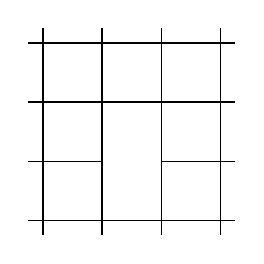
\begin{tikzpicture}[scale=0.75,baseline=(current bounding box.center)]
			%horizontal lines
			\draw (-0.25,0) -- (3.25,0);
			\draw (-0.25,-1) -- (3.25,-1);
			\draw (-0.25,-2) -- (1,-2);
			\draw (2,-2) -- (3.25,-2);
			\draw (-0.25,-3) -- (3.25,-3);
			%vertical lines
			\draw (0,-3.25) -- (0,0.25);
			\draw (1,-3.25) -- (1,0.25);
			\draw (2,-3.25) -- (2,0.25);
			\draw (3,-3.25) -- (3,0.25);
		\end{tikzpicture}
		\caption{One missing qubit defect on a Toric code lattice.}\label{fig:1defect}
	\end{subfigure}\hfill
	\begin{subfigure}[t]{0.2\linewidth}
		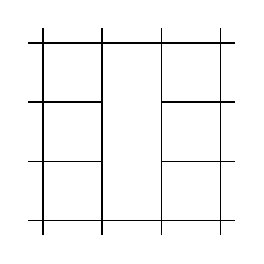
\begin{tikzpicture}[scale=0.75,baseline=(current bounding box.center)]
			%horizontal lines
			\draw (-0.25,0) -- (3.25,0);
			\draw (-0.25,-1) -- (1,-1);
			\draw (2,-1) -- (3.25,-1);
			\draw (-0.25,-2) -- (1,-2);
			\draw (2,-2) -- (3.25,-2);
			\draw (-0.25,-3) -- (3.25,-3);
			%vertical lines
			\draw (0,-3.25) -- (0,0.25);
			\draw (1,-3.25) -- (1,0.25);
			\draw (2,-3.25) -- (2,0.25);
			\draw (3,-3.25) -- (3,0.25);
		\end{tikzpicture}
		\caption{Two adjacent missing qubit defects on a Toric code lattice.}\label{fig:2adjdefects}
	\end{subfigure}\hfill
	\begin{subfigure}[t]{0.2\linewidth}
		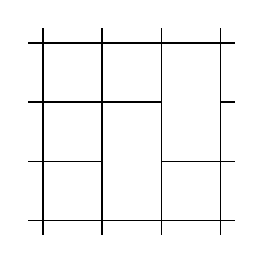
\begin{tikzpicture}[scale=0.75,baseline=(current bounding box.center)]
		%horizontal lines
		\draw (-0.25,0) -- (3.25,0);
		\draw (-0.25,-1) -- (2,-1);
		\draw (3,-1) -- (3.25,-1);
		\draw (-0.25,-2) -- (1,-2);
		\draw (2,-2) -- (3.25,-2);
		\draw (-0.25,-3) -- (3.25,-3);
		%vertical lines
		\draw (0,-3.25) -- (0,0.25);
		\draw (1,-3.25) -- (1,0.25);
		\draw (2,-3.25) -- (2,0.25);
		\draw (3,-3.25) -- (3,0.25);
		\end{tikzpicture}
		\caption{Two distant missing qubit defects on a Toric code lattice.}\label{fig:2distdefects}
	\end{subfigure}
	\caption{Depiction of different situations where missing qubit defects are inserted on a Toric code lattice. In the case of more than one missing link the ground space for the system depends on whether the defects are adjacent to each other or not.}
\end{figure}

We can incorporate such \emph{indirect} dynamical information into our kinematical space $\mathcal{F}_{\le n}(\mathbb{C}^d)$ as follows. We start by writing out 
\begin{equation}
	\mathcal{V}_{\le n}(\mathbb{C}^d) = \bigoplus_{e_1,e_2, \ldots, e_{N^2} =0}^1 \mathcal{V}_{e_1,e_2,\ldots, e_N^2},
\end{equation}
where $\mathcal{V}_{e_1,e_2,\ldots, e_N^2}$ is the ground eigenspace for the toric code with a missing-edge defect at every edge $e_j$ with $e_j=0$. Writing out the first terms of this big direct sum gives us
\begin{equation}
	\mathcal{V}_{\le n}(\mathbb{C}^d) = (\mathbb{C}^2\otimes \mathbb{C}^2)\oplus \mathbb{C}^{N^2}\otimes (\mathbb{C}^2\otimes \mathbb{C}^2\otimes \mathbb{C}^2)\oplus \cdots.
\end{equation}
The first direct summand corresponds to the ground eigenspace of the toric code without defects, the second summand corresponds to the $N^2$ possible single defects, etc.

The full direct-sum structure of $\mathcal{V}_{\le n}(\mathbb{C}^d)$ is not easy to describe. Indeed, this is why we use a category theoretic language to discuss these problems. 

So far, the space $\mathcal{V}_{\le n}(\mathbb{C}^d)$ is the low-energy configuration space for a topologically ordered system, the toric code, on a lattice with an indefinite number of missing-edge defects. In this case, we assume we somehow \emph{can know} where the defects are located. However, for a full dynamical theory, this assumption is potentially unjustified.

To incorporate the effects of such limited detection ability we impose an \emph{equivalence relation} on $\mathcal{V}_{\le n}(\mathbb{C}^d)$ where we identify ``physically indistinguishable'' configurations of defects. There are many possible notions of indistinguishability: this is an \emph{operational} notion and must be justified on a case by case basis. 

One particular, rather coarse, notion of indistinguishability may be justified as follows. Suppose we have a state $|\phi\rangle$ of the system for a defect configuration $e_1,e_2, \ldots, e_{N^2}$ and another $|\psi\rangle$ for a defect configuration with the same number of defects at possible different locations $e_1',e_2',\ldots, e'_{N^2}$. We say that the two states $|\phi\rangle$ and $|\psi\rangle$ are \emph{equivalent} if there is a unitary circuit which can transform $|\phi\rangle$ to $|\psi\rangle$. This, in particular, requires that the subspaces $\mathcal{V}_{e_1,e_2,\ldots,e_{N^2}}$ and $\mathcal{V}_{e_1',e_2',\ldots,e_{N^2}'}$ which contain $|\phi\rangle$ and $|\psi\rangle$ have the same dimensions.

This equivalence relation collapses many of the direct sums appearing in $\mathcal{V}_{e_1,e_2,\ldots,e_{N^2}}$, e.g., after applying the equivalence relation the first two summands above become
\begin{equation}
	\left(\mathcal{V}_{\le n}(\mathbb{C}^d)/\sim\right) = (\mathbb{C}^2\otimes \mathbb{C}^2)\oplus (\mathbb{C}^2\otimes \mathbb{C}^2\otimes \mathbb{C}^2)\oplus \cdots.
\end{equation}

Writing out the whole ground eigenspace and applying the equivalence relation to it results in a highly intricately combinatorial problem, which is why we exploit concepts from category theory to model defects in the system. Of course, the above description is not only restricted to the toric code case. In the next section, we show how ideas and techniques from category theory can be used to model dynamical defects in a system similar to the golden chain \cite{Feiguin2007}, namely a chain with $\Vec(\Z/2\Z)$ fusion rules.

  